\documentclass[aspectratio=169]{beamer}
\usetheme{focus}

%\usepackage{beamerthemesplit}
%\beamertemplatenavigationsymbolsempty
\usepackage{amsmath}
\usepackage{amsthm}
\usepackage{amssymb}
\usepackage{latexsym}
\usepackage{graphicx}
\usepackage{fancybox}
\usepackage{dsfont}
\usepackage{multirow} 
\usepackage{multicol}
\usepackage{booktabs} 
\usepackage{dcolumn}
\usepackage{soul}
\usepackage[cache=false]{minted}
\usepackage{MnSymbol}
\usepackage{stmaryrd}


\DeclareMathOperator*{\argmax}{arg\,max}
\DeclareMathOperator*{\argmin}{arg\,min}

\newcommand{\X}{\mathtt{X}}
\newcommand{\Y}{\mathtt{Y}}

%\newcommand{\R}{\mathbb{R}}
%\newcommand{\E}{\mathbb{E}}
%\newcommand{\V}{\mathbb{V}}
\newcommand{\p}{\mathbb{P}}
\newcommand*\df{\mathop{}\!\mathrm{d}}
\newcommand{\del}{\partial}


% imports
\usepackage{xargs}
\usepackage{xpatch}
\usepackage{etoolbox}
\usepackage{pdflscape}
\usepackage{booktabs}
\usepackage{threeparttable}
\usepackage[skip=0.2\baselineskip]{caption}

% command for inputting raw latex
\makeatletter
\newcommand\primitiveinput[1]{\@@input #1 }
\makeatother

% common table command
\newcommandx{\tablecontent}[4]{
    \begin{threeparttable}[!ht]
        \centering
        \caption{#3}
        \vspace{-1em}
        \footnotesize
        \begin{tabular}{#1}
            \primitiveinput{../tables/#2.tex}
        \end{tabular}
        \vspace{-0.2em}
        \begin{tablenotes}[flushleft]
            #4
        \end{tablenotes}
    \end{threeparttable}
}




% \usepackage{slashbox}
\title{Lecture 2: Basics of Panel Data}
\author{Chris Conlon }
\institute{NYU Stern }


\newcommand{\norm}[1]{\left\lVert#1\right\rVert}
\newcommand{\R}{\mathbb{R}}
\newcommand{\E}{\mathbb{E}}
\newcommand{\V}{\mathbb{V}}
\newcommand{\ol}{\overline}
%\newcommand{\ul}{\underline}
\newcommand{\pp}{{\prime \prime}}
\newcommand{\ppp}{{\prime \prime \prime}}
\newcommand{\policy}{\gamma}


\newcommand{\fp}{\frame[plain]}

\date{\today}

\begin{document}
\maketitle

\begin{frame}[fragile]{Packages for Today}
Let's load some packages so that I can make some better looking plots:\\
\begin{minted}{R}
#always
library(tidyverse)
# for SE's
library(estimatr)
library(broom)
# for Panel
library(lfe)
library(plm)
\end{minted}
\end{frame}


\begin{frame}{Today's Plan}
\begin{itemize}
\item Recap OLS and various forms of standard errors
\item Standard errors are tedious but I guess you are supposed to know this stuff
\item Hopefully first and last time we talk about this
\end{itemize}
\end{frame}


\section{Recap: Asymptotics for OLS and the Linear Model}


\begin{frame}{OLS}
\begin{align*}
y_i = \beta_0 + \beta x_i + u_i
\end{align*}
Recall the three basic OLS assumptions
\begin{enumerate}
\item $E(u_i |X_i ) = 0$
\item $(X_i,Y_i)$, $i =1,\ldots,n$, are i.i.d.
\item Large outliers are rare $E[Y^4]< \infty$ and $E[X^4]<\infty$.
\end{enumerate}
\end{frame}

\begin{frame}{Gauss Markov Theorem}
Gauss Markov Adds two assumptions:
\begin{enumerate}
\item $E(u_i |X_i ) = 0$
\item $(X_i,Y_i)$, $i =1,\ldots,n$, are i.i.d.
\item Large outliers are rare $E[Y^4]< \infty$ and $E[X^4]<\infty$.
\item $Var(u_i) = \sigma^2$ (homoskedasticity)
\item $u_i \sim N(0,\sigma^2)$ (normal errors)
\end{enumerate}
Under these assumptions you learned that OLS is \alert{BLUE}
\end{frame}



\begin{frame}{Outliers and Leverage}
One way to find \alert{outliers} is to calculate the \alert{leverage} of each observation $i$. We begin with the \alert{hat matrix}:
\begin{align*}
P = X  (X'X)^{-1} X'
\end{align*}
and consider the diagonal elements which for some reason are labeled $h_{ii}$
\begin{align*}
h_{ii} = x_i (X'X)^{-1} x_i'
\end{align*}
This tells us how \alert{influential} an observation is in our estimate of $\widehat{\beta}$.\\
Particularly important for $\{0,1\}$ \alert{dummy variables} with uneven groups.
\end{frame}


\begin{frame}{Leave One Out Regression}
\begin{itemize}
\item This is sometimes called the \alert{Jackknife}
\item Sometimes it is helpful to know what would happen if we omitted a single observation $i$
\item Turns out we don't need to run $N$ regressions
\begin{align*}
\widehat{\beta}_{-i} &= (X_{-i}'X_{-i})^{-1} X_{-i}' Y_{-i} \\
&=\widehat{\beta} -  (X 'X)^{-1} x_i  \tilde{u}_i  \quad \mbox{ where } \tilde{u}_i = (1-h_{ii})^{-1}\hat{u}_i
\end{align*}
\item $\tilde{u}_i $ has the interpretation of the \alert{LOO prediction error}.
\item high leverage observations move $\widehat{\beta}$ a lot.
\end{itemize}
You can read more about this in Ch3 of Hansen. [Skip derivation]
\end{frame}

\begin{frame}[fragile]{Leverage and QQ plots}
\begin{minted}{R}
library(car)
fit <- lm(mpg~disp+hp+wt+drat, data=mtcars)

# Assessing Outliers
outlierTest(fit) # Bonferonni p-value for most extreme obs
qqPlot(fit, main="QQ Plot") #qq plot for studentized resid 
leveragePlots(fit) # leverage plots
\end{minted}
\end{frame}

\begin{frame}{Leverage Plot}
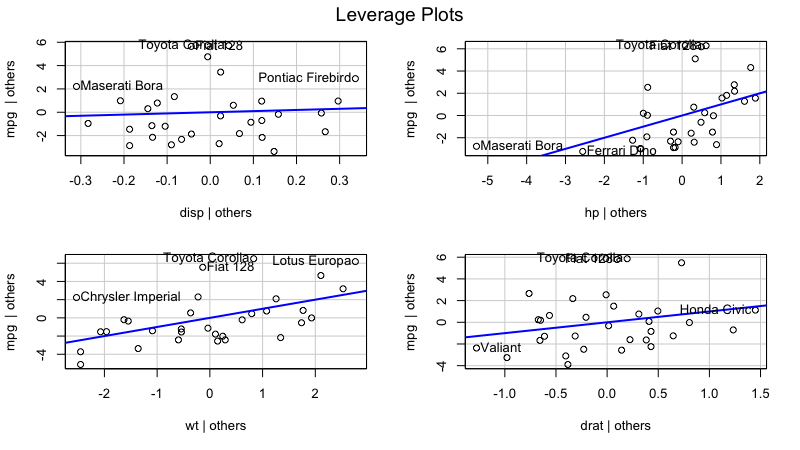
\includegraphics[width=5.5in]{./resources/leverage_plot.png}
\end{frame}



\begin{frame}{Variance of $\widehat{\beta}$}
Start with the variance of the residuals to form a \alert{diagonal} matrix $D$:
\begin{align*}
\operatorname { Var } ( \mathbf{u} | \mathbf { X } ) &= \mathbb { E } \left( \mathbf{u u} ^ { \prime } | \mathbf { X } \right){ = } \mathbf { D }\\
\mathbf { D } &= \operatorname { diag } \left( \sigma _ { 1 } ^ { 2 } , \ldots , \sigma _ { n } ^ { 2 } \right) = \left( \begin{array} { c c c c } { \sigma _ { 1 } ^ { 2 } } & { 0 } & { \cdots } & { 0 } \\ { 0 } & { \sigma _ { 2 } ^ { 2 } } & { \cdots } & { 0 } \\ { \vdots } & { \vdots } & { \ddots } & { \vdots } \\ { 0 } & { 0 } & { \cdots } & { \sigma _ { n } ^ { 2 } } \end{array} \right)
\end{align*}
\begin{itemize}
\item $\mathbf{D}$ is diagonal because $\mathbb { E }[u_i u_j | X] = \mathbb { E }[u_i  | x_i]  \mathbb { E }[u_j  | x_j]=0$ (independence)
\item The elements of $D_i$ are given by $\mathbb { E }[u_i^2 | X] = \mathbb { E }[u_i^2 | x_i] = \sigma_i^2$.
\item In the \alert{homoskedastic} case $\mathbf{D} = \sigma^2 \mathbf{I}_n$.
\end{itemize}
\end{frame}

\begin{frame}{Variance of $\widehat{\beta}$}
A useful identity for linear algebra:
\begin{align*}
\operatorname { Var } (a \mathbf{Z} ) = a^2 \operatorname { Var }(\mathbf{Z})\\
\operatorname { Var } (A \mathbf{Z} ) = A \operatorname { Var }(\mathbf{Z}) A'
\end{align*}

Recall that $\operatorname { Var } ( \mathbf{Y} |\mathbf{X} )  = \operatorname { Var } ( \mathbf{u} | \mathbf { X } ) $ and also
recall the formula for $\widehat{\beta}$:
\begin{align*}
\widehat{\beta} &= \underbrace{(X'X)^{-1} X' }_{A} Y= A' Y \\
\mathbf{V}_{\widehat{\beta}} = \operatorname { Var }(\widehat{\beta} | X)&= (X'X)^{-1} X'  \operatorname { Var }(Y| X) X (X'X)^{-1} \\
													     &= (X'X)^{-1} (X'  \mathbf{D} X) (X'X)^{-1} 
\end{align*}
We have that $ (X'  \mathbf{D} X)  = \sum_{i=1}^N x_i x_i'\sigma_i^2$. Under homoskedasticity $\mathbf{D} = \sigma^2 \mathbf{I}_n$ and $\mathbf{V}_{\widehat{\beta}} = \sigma^2 (X'X)^{-1}$.
\end{frame}


\begin{frame}{Variance of $\widehat{\beta}$}
\begin{align*}
\mathbf { D } = \operatorname { diag } \left( \sigma _ { 1 } ^ { 2 } , \ldots , \sigma _ { n } ^ { 2 } \right)
= \mathbb { E } \left( u_i u_i'  | \mathbf { X } \right)
= \mathbb { E } \left( \widetilde{\mathbf{D}}| \mathbf { X } \right)
\end{align*}

We can estimate $\widehat{\mathbf{V}}_{\widehat{\beta}}$ by plugging in $\mathbf{D} \rightarrow  \widetilde{\mathbf{D}} $:
\begin{align*}
\mathbf{V}_{\widehat{\beta}} &= (X'X)^{-1} (X'  \widetilde{\mathbf{D}} X) (X'X)^{-1} \\
&= (X'X)^{-1} \left(\sum_{i=1}^N x_i x_i' u_i^2  \right) (X'X)^{-1} 
\end{align*}
The expectation shows us this estimator is unbiased:
\begin{align*}
E[\mathbf{V}_{\widehat{\beta}} | X]
&= (X'X)^{-1} \left(\sum_{i=1}^N x_i x_i' E[u_i^2 | X] \right) (X'X)^{-1} \\
&= (X'X)^{-1} \left(\sum_{i=1}^N x_i x_i' \sigma_i^2 \right) (X'X)^{-1} = (X'X)^{-1} (X' D X) (X'X)^{-1} 
\end{align*}
\end{frame}



\begin{frame}{Heteroskedasticity Consistent (HC) Variance Estimates}
What we need is a consistent estimator for $\hat{u}^2_i$.
\begin{align*}
\mathbf{V}_{\widehat{\beta}}^{HC0}&= (X'X)^{-1} \left(\sum_{i=1}^N x_i x_i' \hat{u}_i^2 \right) (X'X)^{-1} \\
\mathbf{V}_{\widehat{\beta}}^{HC1}&= (X'X)^{-1} \left(\sum_{i=1}^N x_i x_i' \hat{u}_i^2 \right) (X'X)^{-1} \cdot \left(\frac{n}{n-k}  \right)
\end{align*}
Could use $\tilde{u}_i$ instead of $\hat{u}_i$ for a better estimate
\begin{align*}
\mathbf{V}_{\widehat{\beta}}^{HC2}&= (X'X)^{-1} \left(\sum_{i=1}^N (1-h_{ii})^{-1} x_i x_i' \hat{u}_i^2 \right) (X'X)^{-1} \\
\mathbf{V}_{\widehat{\beta}}^{HC3}&= (X'X)^{-1} \left(\sum_{i=1}^N (1-h_{ii})^{-2} x_i x_i' \hat{u}_i^2 \right) (X'X)^{-1} \\
\end{align*}
\end{frame}

\begin{frame}{Heteroskedasticity Consistent (HC) Variance Estimates}
\begin{itemize}
\item We know that $\mathbf{V}_{\widehat{\beta}}^{HC3} > \mathbf{V}_{\widehat{\beta}}^{HC2} > \mathbf{V}_{\widehat{\beta}}^{HC0}$ because $(1- h_{ii}) <1$.
\item $HC3$ are the most \alert{conservative} and also place the most weight on potential outliers.
\item \texttt{Stata} uses $HC1$ as the default and it is what most people refer to when they say \alert{robust standard errors}.
\item These are often called White (1980) SE's or Eicher-Huber-White SE's.
\item In small sample some evidence that $HC2$ does better.
\end{itemize}
\end{frame}

\begin{frame}[fragile]{Heteroskedasticity Consistent (HC) Variance Estimates}
\footnotesize
To read about SE's in \texttt{estimatr}:
\url{ https://declaredesign.org/r/estimatr/articles/mathematical-notes.html}
\begin{minted}{R}
dat <- data.frame(X = matrix(rnorm(2000*5), 2000), y = rnorm(2000))
hc0<-lm_robust(y ~ ., data = dat, se_type="HC0")$std.error
hc1<-lm_robust(y ~ ., data = dat, se_type="HC1")$std.error
hc2<-lm_robust(y ~ ., data = dat, se_type="HC2")$std.error
hc3<-lm_robust(y ~ ., data = dat, se_type="HC3")$std.error
all(hc2 > hc0 )
[1] TRUE
all(hc3> hc2 )
[1] TRUE
\end{minted}
\end{frame}

\begin{frame}{What is Clustering?}
Suppose we want to relax our i.i.d. assumption:
\begin{itemize}
\item Each observation $i$ is a \alert{villager} and each group $g$ is a \alert{village}
\item Each observation $i$ is a \alert{student} and each group $g$ is a \alert{class}.
\item Each observation $t$ is a \alert{year} and each entity $i$ is a \alert{state}.
\item Each observation $t$ is a \alert{week} and each entity $i$ is a \alert{shopper}.
\end{itemize}
We might expect that $\operatorname { Cov } (u_{g1},u_{g2},\ldots,u_{gN}) \neq 0 \rightarrow$ independence is a bad assumption. 
\end{frame}

\begin{frame}{Clustering: Intuition}
The groups (villages, classrooms, states) are independent of one another, but within each group we can allow for arbitrary correlation.
\begin{itemize}
\item If correlation is within an individual overtime we call it \alert{serial correlation} or \alert{autocorrelation}
\item Just like in time-series$\rightarrow$ we have fewer effective independent observations in our sample.
\item Asymptotics now about the number of groups $G \rightarrow \infty$ not observations $N \rightarrow \infty$
\end{itemize}
\end{frame}

\begin{frame}{Clustering}
Begin by stacking up observations in each group $\mathbf{y}_{g }  = [y_{g1},\ldots,y_{g n_g}]$, we can write OLS three ways:
\begin{align*}
y_{ig } &= x_{ig}' \beta + u_{ig}\\
\mathbf{y}_{g } &= \mathbf{X}_{g} \beta + \mathbf{u}_{g}\\
\mathbf{Y} &= \mathbf{X} \beta + \mathbf{u}
\end{align*}
All of these are equivalent:
\begin{align*}
\widehat {  \beta  } &= \left( \sum _ { g = 1 } ^ { G } \sum _ { i = 1 } ^ { n _ { g } } x _ { i g }' { x } _ { i g } \right) ^ { - 1 } \left( \sum _ { g = 1 } ^ { G } \sum _ { i = 1 } ^ { n _ { g } } x _ { i g }' y _ { i g } \right)\\
\widehat {  \beta  }  &=  \left(  \sum _ { g = 1 } ^ { G } \mathbf{X}_g' \mathbf{X}_g \right)^{-1} \left(  \sum _ { g = 1 } ^ { G } \mathbf{X}_g' \mathbf{y}_g \right)\\
\widehat {  \beta  }  &=  \left( \mathbf{X}' \mathbf{X} \right)^{-1} \left(   \mathbf{X}' \mathbf{Y} \right)\\
\end{align*}
\end{frame}

\begin{frame}{Clustering (Continued)}
The error terms have covariance within each cluster $g$ as:
\begin{align*}
 \boldsymbol{\Sigma}_ { g } = \mathbb { E } \left( \mathbf{u} _ { g }  \mathbf{ u } _ { g } ^ { \prime } | \boldsymbol { X } _ { g } \right)
\end{align*}

In order to calculate $\widehat{V}_{\widehat{\beta}}$ we replace the covariance matrix $\mathbf{D}$ with $\Omega$ and consider an estimator $\widehat{\Omega}_n$. We exploit \alert{independence across clusters}:
\begin{align*}
\operatorname { var } \left( \left( \sum _ { g = 1 } ^ { G } \boldsymbol { X } _ { g } ^ { \prime } \mathbf{u}_ { g } \right) | \boldsymbol { X } \right) = \sum _ { g = 1 } ^ { G } \operatorname { var } \left( \boldsymbol { X } _ { g } ^ { \prime } \boldsymbol { u } _ { g } | \boldsymbol { X } _ { g } \right)
= \sum _ { g = 1 } ^ { G } \boldsymbol { X } _ { g } ^ { \prime } \mathbb { E } \left( \boldsymbol { u } _ { g } \boldsymbol { u } _ { g } ^ { \prime } | \boldsymbol { X } _ { g } \right) \boldsymbol { X } _ { g }
= \sum _ { g = 1 } ^ { G } \boldsymbol { X } _ { g } ^ { \prime } \boldsymbol { \Sigma } _ { g } \mathbf { X } _ { g } 
 \equiv \Omega_N
\end{align*}
And an estimate of the variance:
\begin{align*}
\boldsymbol { V } _ { \widehat { \boldsymbol { \beta } } } = \operatorname { var } ( \widehat { \boldsymbol { \beta } } | \boldsymbol { X } )
= \left( \mathbf { X } ^ { \prime } \mathbf { X } \right) ^ { - 1 } \boldsymbol { \Omega } _ { n } \left( \mathbf { X } ^ { \prime } \mathbf { X } \right) ^ { - 1 }
\end{align*}
\end{frame}


\begin{frame}{Clustered SE's}
\begin{align*}
\widehat { \Omega } _ { n } &= \sum _ { g = 1 } ^ { G } X _ { g } ^ { \prime } \widehat {\mathbf{ u }} _ { g }\widehat {\mathbf{ u }}_{g} ^ { \prime } X _ { g }\\
&= \sum _ { g = 1 } ^ { G } \sum _ { i = 1 } ^ { n _ { g } } \sum _ { \ell = 1 } ^ { n _ { g } } x _ { i g } x _ { \ell g } ^ { \prime } \widehat { u } _ { i g } \widehat { u } _ { \ell g }\\
&= \sum _ { g = 1 } ^ { G } \left( \sum _ { i = 1 } ^ { n _ { g } } x _ { i g } \widehat { u } _ { i g } \right) \left( \sum _ { \ell = 1 } ^ { n _ { g } } x _ { \ell g } \widehat { u } _ { \ell g } \right) ^ { \prime }
\end{align*}
\begin{itemize}
\item First line makes explicit: independence over each of $G$ clusters
\item Last line easiest for computer
\end{itemize}
\end{frame}

\begin{frame}{Clustered SE's}
\begin{align*}
\widehat { \boldsymbol { V } } _ { \hat { \beta } } ^ { \mathrm { CR } 1 } = \left( \boldsymbol { X } ^ { \prime } \boldsymbol { X } \right) ^ { - 1 } \left( \sum _ { g = 1 } ^ { G } \boldsymbol { X } _ { g } ^ { \prime } \widehat { u } _ { g } \widehat { \boldsymbol { u } } _ { g } ^ { \prime } \boldsymbol { X } _ { g } \right) \left( \boldsymbol { X } ^ { \prime } \boldsymbol { X } \right) ^ { - 1 }\\
\widehat { \boldsymbol { V } } _ { \hat { \beta } } ^ { \mathrm { CR } 3 } = \left( \boldsymbol { X } ^ { \prime } \boldsymbol { X } \right) ^ { - 1 } \left( \sum _ { g = 1 } ^ { G } \boldsymbol { X } _ { g } ^ { \prime } \widetilde { u } _ { g } \widetilde { \boldsymbol { u } } _ { g } ^ { \prime } \boldsymbol { X } _ { g } \right) \left( \boldsymbol { X } ^ { \prime } \boldsymbol { X } \right) ^ { - 1 }
\end{align*}
\begin{itemize}
\item Can replace  $\hat { \mathbf{u}}_g  \rightarrow \tilde { \mathbf{u}}_g $ for leave-one out like $HC3$ (these are called $CR3$).
\end{itemize}
\end{frame}


\begin{frame}[fragile]{Clustering in R}
\begin{minted}{R}
lm_robust(y~ x1 + x2, data=df, se_type="CR0", cluster=group_id )
lm_robust(y~ x1 + x2, data=df, se_type="CR2", cluster=group_id )
lm_robust(y~ x1 + x2, data=df, se_type="CR1", cluster=group_id )
\end{minted}
\end{frame}


\begin{frame}{Most Asked PhD Student Econometric Question}
 How should I cluster my standard errors?
\begin{itemize}
\item Heck if I know.
\item This is very problem specific
\item It matters a lot $\rightarrow$ standard errors can get orders of magnitude larger.
\item Do you believe across group independence or not? [this is the only thing that matters]
\item If you include \alert{fixed effects} probably you need at least clustering at that level.
\end{itemize}
\end{frame}


\begin{frame}{Newey West Standard Errors (HAC)}
\begin{itemize}
\item In serially correlated data we need to account for $\operatorname{ Cov } (u_{t},u_{t-1},\ldots ) \neq 0$.
\item Clustering is one solution, but we may end up throwing away all of our data.
\item Instead we could estimate the serial correlation.
\item May also want standard errors that are \alert{heteroskedasticity AND autocorrelation consistent} (HAC).
\item Have to select a number of lags $L$
\end{itemize}
\begin{align*}
\widehat { \Omega } _ { n,L }^{HAC} &= \sum _ { t = 1 } ^ { T }  u _ { t }^2 x_t x_t'  + \sum_{l=1}^L \sum _ { t = l+1 } ^ { T } w_l u_t u _ { t-l } \left( x_t x_{t-l}' +  x_{t-l} x_{t}'  \right)\\
w_l &= 1 - \frac{l}{L+1}
\end{align*}
\end{frame}




\begin{frame}{What about $\beta$?}
\begin{itemize}
\item All of the estimates above should produce \alert{identical} point estimates
\item We have just been talking about adjusting \alert{standard errors}
\item Should the presence of heteroskedasticity change our estimates of $\widehat{\beta}$ as well?
\end{itemize}
\end{frame}



\begin{frame}{OLS and WLS}
A simple extension is Weighted Least Squares (WLS)
\begin{itemize}
\item Different motivations
\item Suppose we have sampling weights that are not $\frac{1}{n}$ from survey data, etc:
    \begin{itemize}
    \item If my population is supposed to represent all US residents and my sample is 75\% Women...
    \item Relax LSA (2) $(X_i,Y_i)$, $i =1,\ldots,n$, are i.i.d.
\end{itemize}
\item In this case, OLS is still unbiased and consistent, just \alert{inefficient}
\end{itemize}
\end{frame}

\begin{frame}{WLS}
Can weight each observation as $w_i$ so that $\sum_{i=1}^N w_i = 1$ instead of $w_i=\frac{1}{N}$.\\
Can define a diagonal matrix $W$ with entries $w_i$.
\begin{align*}
\arg \min_{\beta} \sum_{i=1}^N w_i (y_i - X_i \beta)^2 = \arg \min_{\beta} \norm{W^{1/2}|Y - X \beta| } 
\end{align*}
Can also consider a transformation of the data 
\begin{align*}
\tilde{y}_i &= \sqrt{w}_i y_i , \quad  \tilde{x}_i = \sqrt{w}_i x_i \\\
\tilde{Y} &= W^{1/2} Y, \quad  \tilde{X} = W^{1/2} X
\end{align*}
A regression of $\tilde{Y}$ on $\tilde{X}$:
\begin{align*}
\widehat{\beta}_{WLS} = (\tilde{X}'\tilde{X})^{-1}\tilde{X}'\tilde{Y} = (X' W X)^{-1} X' W Y
\end{align*}
\end{frame}

\begin{frame}{WLS}
Also used as a solution to heteroskedasticity
\begin{itemize}
    \item Relax LSA (2) $(X_i,Y_i)$, $i =1,\ldots,n$, are i.i.d.
    \item Relax LSA (4) $Var(u_i) = \sigma^2$ (homoskedasticity)
\end{itemize}
Why? We are minimizing weighted sum of squared residuals:
\begin{align*}
\sum_{i=1}^N w_i (y_i - \hat{y}_i)^2 = \sum_{i=1}^N w_i \varepsilon_i^2 
\end{align*}
Suppose we have heteroskedasticity so that $Var(\varepsilon_i) = \sigma_i^2$ and $w_i \propto \frac{1}{\sigma_i^2}$.\\
In this setting WLS is \alert{BLUE}.
\end{frame}

\begin{frame}{WLS}
Why does anyone ever run OLS instead of WLS?
\begin{itemize}
\item Problem is that $\sigma_i^2$ is unknown before we run our regression.
\item We can estimate $\widehat{\sigma}_i^2$.
\end{itemize}
This procedure is known as Iteratively Re-weighted Least Squares \alert{IRLS}
\begin{enumerate}
\item Intialize weights to identity matrix: $W = I$
\item Regress $Y$ on $X$ with weights $W$
\item Obtain $\widehat{\varepsilon}_i$.
\item Update $W$ with $w_{ii} = \frac{1}{\widehat{\varepsilon}_i^2}$
\item Repeat until parameter estimates don't change
\end{enumerate}
\end{frame}



\begin{frame}{GLS and FGLS}
There is no reason to require that $W$ be diagonal. This gives us \alert{Generalized Least Squares}
\begin{align*}
\widehat{\beta}_{GLS} = (\tilde{X}'\tilde{X})^{-1}\tilde{X}'\tilde{Y} = (X' \Omega  X)^{-1} \Omega' W Y
\end{align*}
The idea is to use the \alert{inverse covariance matrix} of residuals. But this is high dimensional $(N \times N)$ and estimating it is harder than our original problem!

 Feasible Generalized Least Squares \alert{FGLS}:
\begin{enumerate}
\item Intialize weights to identity matrix: $\widehat{\Omega}= I$
\item Regress $Y$ on $X$ with weighting matrix $\widehat{\Omega}$
\item Obtain $\widehat{\varepsilon}_i$.
\item Construct $E[ \varepsilon_i^2 | X, Z]$ via (nonlinear) regression: $\exp[ \gamma_0 + \gamma_1 x_{i} + \gamma_2 z_{i}]$.
\item Update $\widehat{\Omega}$ with $E[ \varepsilon_i^2 | X, Z]$
\item Repeat until parameter estimates don't change
\end{enumerate}
\end{frame}



\section{What is Panel Data?}


\begin{frame}{Big Picture}
We can combine cross sectional analysis and time series analysis to form \alert{panel data}.
\begin{itemize}
\item Now $y_{it}$ and $x_{it}$ have two subscripts:
\begin{itemize}
\item $i$ for \alert{individual} or \alert{entity}
\item $t$ for \alert{time}
\end{itemize}
\item It used to be that panel data was rare enough that it was a separate set of topics within econometrics. Now it is the norm.
\item The main similarity to \alert{time series} is that observations within an individual are \alert{correlated} with one another
\item The main similarity to \alert{cross sectional} econometrics is that individuals are often treated as \alert{independent}.
\end{itemize}
\end{frame}

\begin{frame}{Terminology}
\begin{description}
\item[Longitudinal data] another term for panel data (especially in demography/sociology)
\item[Repeated cross section] not a panel, but a data structure with multiple
individuals observed in each of multiple time periods. In contrast to panel data,
we don't observe the same individuals in multiple time periods. 
\item[Balanced panel] each of $n$ individuals is observed $T$ times, usually
    over the same time period
\item[Unbalanced panel] at least of the individuals are not observed in every period.
    Sometimes unbalanced panels result from sampling designs, and sometimes they
    are a result of entry/exit or birth/death
\item[Sparse Panel] very little overlap between $(i,j)$. Think about matched firm-worker datasets (nobody works at every firm!)
\item[Wide Panel]has many individuals (large $n$); a
\item[Long Panel] has many time periods (large $T$). The asymptotic properties of an estimator can be different
 when $n \rightarrow \infty$ as opposed to $T \rightarrow \infty$
\end{description}
\end{frame}




\begin{frame}{Basics of Panel Data}
Often interested in a regression of the form:
\begin{align*}
y_{it} = \beta_i x_{it} + c_i + u_{it} \quad i=1,\ldots,N \quad t=1,\ldots,T
\end{align*}
\begin{itemize}
\item With \alert{repeated observations} on the same individual the assumption that $u_{it}$ is I.I.D. is unrealistic $\rightarrow$ will need to adjust standard errors.
\item Why? This year's outcome is likely related to last year's outcome...
\item But with repeated observations on an individual we can control for a great deal of \alert{unobserved heterogeneity} or omitted variables.
\item We may want to include lagged $y_{i,t-1}$ as a regressor in \alert{dynamic panel} models.
\end{itemize}
\end{frame}


\begin{frame}{Basics of Panel Data}
\begin{align*}
y_{it} = \beta_i x_{it} + c_i + u_{it} \quad i=1,\ldots,N \quad t=1,\ldots,T
\end{align*}
\begin{itemize}
\item Full homogeneity (\alert{Pooled}): $\beta_i = \beta$ $c_i = c$ for all $i$. 
\item \alert{Individual Effects}: $\beta_i = \beta$ for all $i$.
\item \alert{Full heterogeneity} $(\beta_i,c_i)$ are all different (potentially).
\end{itemize}
\end{frame}


\begin{frame}{The Pooled Model}
\begin{align*}
y_{it} = \beta x_{it} + c + u_{it} \quad i=1,\ldots,N \quad t=1,\ldots,T
\end{align*}
\begin{itemize}
\item Requires that $E[x_{it}' u_{it}]=0$ or that $E[ e_{it} | \mathbf{X}_i]=0$.
\item Is this reasonable? Usually not
\end{itemize}
\end{frame}

\begin{frame}{Individual Effects Models}
\begin{align*}
y_{it} = \beta x_{it} + c_i + u_{it} \quad i=1,\ldots,N \quad t=1,\ldots,T
\end{align*}
Now we assume that $(\mathbf{y_i},\mathbf{X_i})$ are i.i.d across $i$ but not necessarily $t$ with $\mathbf{X}_i=[X_{i1},X_{i2},\ldots,X_{iT}]$
Two well known cases:
\begin{description}
    \item[Fixed Effects] $E[u_{it}| \mathbf{X}_i , c_i] = 0$ conditional on FE, we have \alert{conditional mean independence}
    \begin{itemize}
        \item Mostly about solving \alert{Omitted Variable Bias} problem
        \item \alert{Unbiasedness} and \alert{Consistency}
    \end{itemize}
    \item[Random Effects] $E[c_i | \mathbf{X}_i] = 0$ individual effects are uncorrelated with information about individual $i$
    \begin{itemize}
        \item These are really about \alert{heteroskedasticity} and \alert{efficiency}
        \item The point estimates $\widehat{\beta}$ still change though (for same reason as WLS or GLS)
    \end{itemize}
\end{description}
\end{frame}

\begin{frame}{Random Effects}
\begin{align*}
y_{it} = \beta x_{it} + c_i + u_{it}
\end{align*}
\begin{itemize}
    \item Not as popular in econometrics as they used to be
    \item \alert{Efficiency} isn't the big concern, \alert{unbiasedness} is
    \item We usually have enough data that reducing your SE's by 10\% isn't an issue. 
    \item Idea: re-scale the data so that it has \alert{spherical variance} $\sigma^2 \cdot \mathbf{I}_N$
\end{itemize}
\end{frame}


\begin{frame}{How are Random Effects Estimated?: FGLS}
Step 1: Estimate the \alert{pooled regression}
\begin{align*}
y_{it} = \beta x_{it} + e_{it}
\end{align*}
Step 2: calculate means and variances:
\begin{align*}
\footnotesize
\hat { \sigma } _ { e } ^ { 2 } &= \frac { 1 } { N T } \sum _ { i = 1 } ^ { T } \sum _ { t = 1 } ^ { T } \hat { e } _ { i t } ^ { 2 }\\
\hat { c } _ { i } &= \frac { 1 } { T } \sum _ { t = 1 } ^ { T } \hat { e } _ { i t } , \quad \hat { u } _ { i t } = \hat { e } _ { i t } - \hat {c } _ { i }\\
\hat { \sigma } _ { c } ^ { 2 } &= \frac { 1 } { N } \sum _ { i = 1 } ^ { N } \left( \hat { c } _ { i } - \frac { 1 } { N } \sum _ { i = 1 } ^ { N } \hat { c } _ { i } \right) ^ { 2 }\\
\hat { \sigma } _ { u } ^ { 2 } &= \frac { 1 } { N T } \sum _ { i = 1 } ^ { N } \sum _ { t = 1 } ^ { T } \left( \hat { u } _ { i t } - \frac { 1 } { N T } \sum _ { i = 1 } ^ { N } \sum _ { t = 1 } ^ { T } \hat { u } _ { i t } \right) ^ { 2 }
\end{align*}
\end{frame}

\begin{frame}{How are Random Effects Estimated?: FGLS}
Step 3: Update the Matrix $\widehat{\Omega}$
\begin{align*}
\hat { \Omega }_{RE} = \left[ \begin{array} { c c c c } { \hat { \sigma } _ { c } ^ { 2 } + \hat { \sigma } _ { u } ^ { 2 } } & { \hat { \sigma } _ { c } ^ { 2 } } & { \cdots } & { \hat { \sigma } _ { c } ^ { 2 } } \\ { \hat { \sigma } _ { c } ^ { 2 } } & { \hat { \sigma } _ { c } ^ { 2 } + \hat { \sigma } _ { u } ^ { 2 } } & { \cdots } & { \vdots } \\ { \vdots } & { \vdots } & { \ddots } & { \vdots } \\ { \hat { \sigma } _ { c } ^ { 2 } } & { \hat { \sigma } _ { c } ^ { 2 } } & { \cdots } & { \hat { \sigma } _ { c } ^ { 2 } + \hat { \sigma } _ { u } ^ { 2 } } \end{array} \right]
\end{align*}
Step 4: Caclulate the (F)GLS estimator:
\begin{align*}
\hat { \beta} _ { \mathrm { RE } } = \left( \sum _ { i = 1 } ^ { N } \mathbf{X} _ { i } ^ { \prime } \hat { \Omega }_{RE} ^ { - 1 } \mathbf{X} _ { i } \right) ^ { - 1 } \left( \sum _ { i = 1 } ^ { N } \mathbf{X} _ { i } ^ { \prime } \hat { \Omega }_{RE} ^ { - 1 } \mathbf{Y} _ { i } \right)
\end{align*}
\end{frame}


\begin{frame}{How are Random Effects Estimated?: MLE}
\begin{itemize}
\item For a number of reasons most software for random effects doesn't do FGLS
\item \texttt{plm} does this \url{https://cran.r-project.org/web/packages/plm/vignettes/plmPackage.html}
\item It usually assumes that $c_i \sim N(0,\sigma_c^2)$ and $u_{it} \sim N(0,\sigma_u^2)$
\item In this world it is easy to do MLE.
\item The package I will show you \texttt{lme4} does this. \url{https://cran.r-project.org/web/packages/lme4/vignettes/lmer.pdf}
\end{itemize}
\end{frame}


\begin{frame}[fragile]{Random Effects in R}
\begin{minted}{R}
#load libraries
library(lme4)
library(ggplot2)
library(reshape2)

#load example data
data("sleepstudy")

#a simple example
m_avg <- lmer(Reaction ~ 1 + (1|Subject),sleepstudy) 

# see the Random Effects
ranef(m_avg)
\end{minted}
\end{frame}

\begin{frame}[fragile]{Random Effects in R}
\begin{minted}{R}
#to get the fitted average reaction time per subject
reaction_subject <- fixef(m_avg) + ranef(m_avg)$Subject
reaction_subject$Subject<-rownames(reaction_subject)
names(reaction_subject)[1]<-"Intercept"
reaction_subject <- reaction_subject[,c(2,1)]
#plot
ggplot(reaction_subject,aes(x=Subject,y=Intercept))+geom_point()
\end{minted}
\end{frame}


\begin{frame}%{Random Effects in R}
\begin{center}
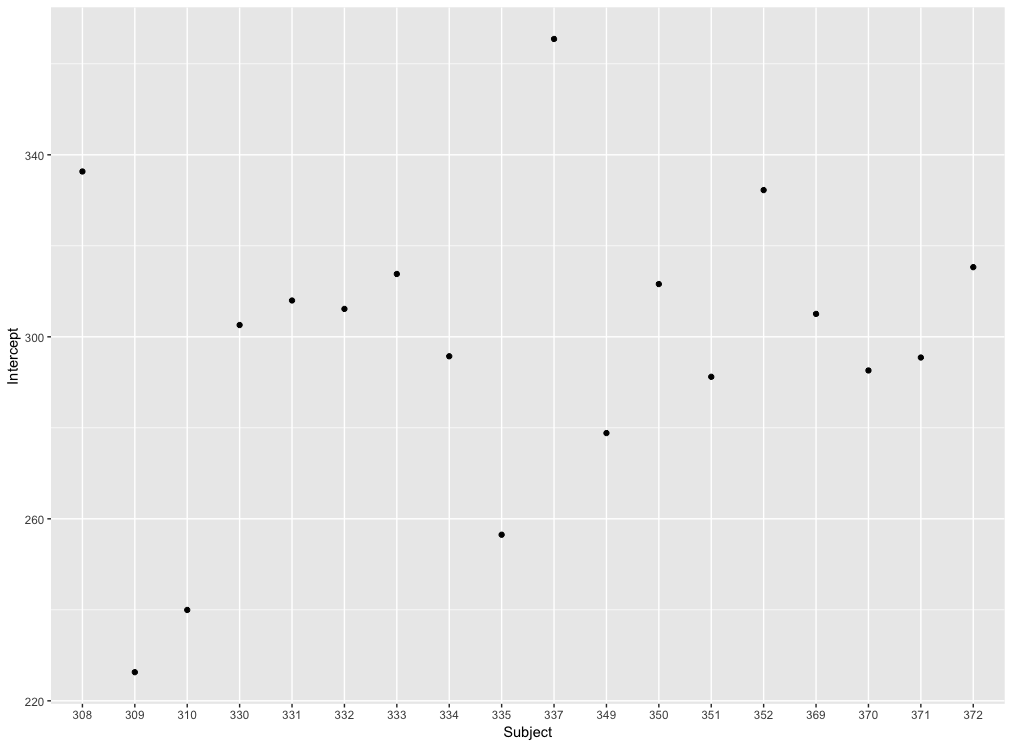
\includegraphics[width=4.5in]{./resources/random_intercepts.png}
\end{center}
\end{frame}

\begin{frame}[fragile]{Random Effects in R}
\footnotesize
\begin{minted}{R}
#This line create a dataframe for 18 hypothetical new subjects
#taking the estimated standard deviation reported in
#summary(m_avg)
new_subject <- data.frame(Subject = as.character(400:417),
  Intercept= fixef(m_avg)+rnorm(18,0,35.75),Status="Simulated")
reaction_subject$Status <- "Observed"
reaction_subject <- rbind(reaction_subject,new_subject)
#new plot
ggplot(reaction_subject,aes(x=Subject,y=Intercept,color=Status))+
  geom_point()+
  geom_hline(aes(yintercept = fixef(m_avg)[1],linewidth=1.5))

\end{minted}
\end{frame}

\begin{frame}%{Random Effects in R}
\begin{center}
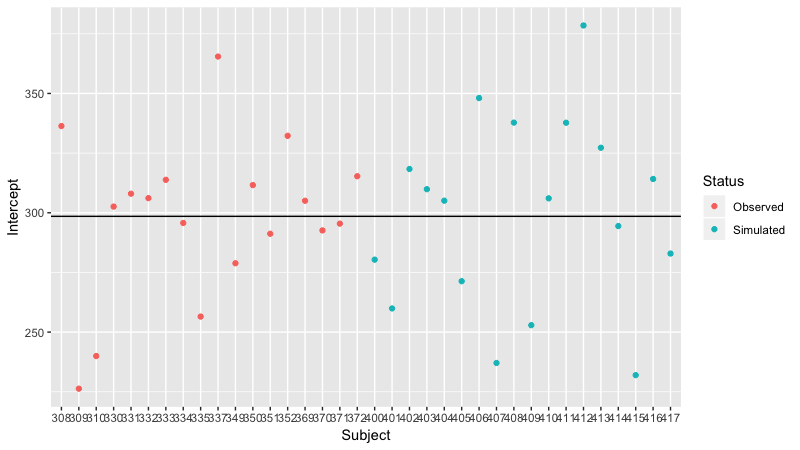
\includegraphics[width=5in]{./resources/random_intercepts2.png}
\end{center}
\end{frame}

\begin{frame}{Random Slope and Intercept / Random Coefficients}
\begin{align*}
y_{it} = \beta_i x_{it} + c_i + u_{it}
\end{align*}
\begin{itemize}
\item Can add a random slope term $\beta_i$ as well
\item This starts to get more useful
\item Parametric restrictions $\beta_i \sim N(0,\sigma_b^2)$ prevent $\beta_i$ realizations from getting too crazy.
\item Later we will think about parametrizing this further $\beta_i(z_i)$
\end{itemize}
\end{frame}




\begin{frame}[fragile]{Random Slope and Intercept R}
\tiny
\begin{minted}{R}
#fit the model
m_slp <- lmer(Reaction ~ Days + (Days | Subject), sleepstudy)
#the next line put all the estimated intercept and slope per
#subject into a dataframe
reaction_slp <- as.data.frame(t(apply(ranef(m_slp)$Subject,
  1,function(x) fixef(m_slp) + x)))
#to get the predicted regression lines we need one further
#step, writing the linear equation: Intercept + Slope*Days
#with different coefficient for each subject
pred_slp <- melt(apply(reaction_slp,1,function(x) x[1] + x[2]*0:9),
  value.name = "Reaction")
#some re-formatting for the plot
names(pred_slp)[1:2] <- c("Days","Subject")
pred_slp$Days <- pred_slp$Days - 1
pred_slp$Subject <- as.factor(pred_slp$Subject)

#plot with actual data
ggplot(pred_slp,aes(x=Days,y=Reaction,color=Subject))+
  geom_line()+
  geom_point(data=sleepstudy,aes(x=Days,y=Reaction))+
  facet_wrap(~Subject,nrow=3)
\end{minted}
\end{frame}

\begin{frame}%{Random Effects in R}
\begin{center}
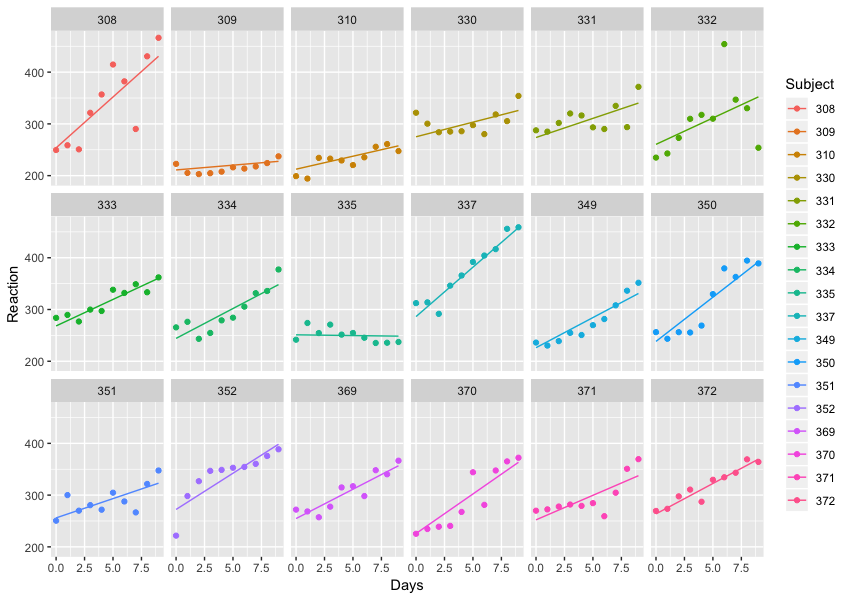
\includegraphics[width=4.8in]{./resources/random_slope_intercept.png}
\end{center}
\end{frame}

\begin{frame}{Control Variables vs. Variables of Interest}
We call a variable $W_i$ a control variable if:
\begin{align*}
E[u_i | X_i, W_i] = E[u_i | W_i]
\end{align*}
Consider the regression model
\begin{align*}
Y_i = \beta_0 + \beta_1 X_i + \beta_2 W_i + u_i
\end{align*}
\begin{itemize}
    \item $\beta_1$ has an interpreation
    \item $\widehat{\beta}_1$ is unbiased
    \item $\widehat{\beta}_2$ is potentially biased: something omitted might be correlated with $W_i$ and a determinant of $Y_i$. 
\end{itemize}
\end{frame}


\begin{frame}{Fixed Effects}
We could think about the same model but now instead of being part of the \alert{residual} $c_i$ is a dummy variable that we want to estimate a (fixed) coefficient on
\begin{align*}
y_{it} = \beta x_{it} + c_i + u_{it}
\end{align*}
Now we require that $E[u_{it}| \mathbf{X}_i , c_i] = 0$
\begin{itemize}
    \item Conditional on observing $c_i$ we have conditional mean independence property satisfied again.
    \item $c_i$ is just a conventional omitted variable: without it our estimate is \alert{biased}, include it in the regression and everything is fine.
\end{itemize}
\end{frame}


\begin{frame}{Fixed Effects as Controls}
\begin{align*}
y_{it} = \beta x_{it} + c_i + u_{it}
\end{align*}
A weaker condition is $E[u_{it}| \mathbf{X}_i , c_i] = E[u_{it}| c_i]$ but allowing $E[u_{it}| \mathbf{X}_i , c_i]\neq 0$
\begin{itemize}
\item Now the fixed effect functions only as a \alert{control}
\item We can't interpret $c_i$ directly, it just proxies for all of the things we don't see
\item Our estimates of $\hat{c}_i$ may be biased, but our estimtes of $\beta$ remain \alert{unbiased}.
\item There is \alert{NO} causal interpretation of fixed effects unless \alert{all variables} correlated with $Y_i$ and $c_i$ are in the regression equation.
\end{itemize}
\end{frame}

\begin{frame}{Fixed Effects: Within Estimator}
The fixed effects estimator
\begin{align*}
y_{it} = \beta x_{it} + c_i + u_{it}
\end{align*}
Is equivalent to the \alert{within estimator} 
\begin{align*}
(y_{it} - \overline{y}_i) = \beta (x_{it} - \overline{x}_i) + (u_{it} - \overline{u}_i)
\end{align*}
You should have learned about this last semester.\\
Also known as \alert{Absorb} / \alert{ Difference Out} / \alert{ Within Transform}
\end{frame}

\begin{frame}{Fixed Effects: LSDV Estimator}
The fixed effects estimator
\begin{align*}
y_{it} = \beta x_{it} + c_i + u_{it}
\end{align*}
Is also equivalent to the least squres dummy variables (LSDV) regression:
\begin{align*}
y_{it} = \beta x_{it} + \sum_{i=1}^N \gamma_i \cdot \mathbf{I}_{i} + u_{it}
\end{align*}
You should have learned about this last semester.
\end{frame}


\begin{frame}{Fixed Effects: Multicolinearity}
If we include a dummy (or fixed effect for every state we cannot estimate a constant term)
\begin{align*}
y_{it} = \alert{\beta_0} + \beta x_{it} + c_i + u_{it}
\end{align*}
\begin{itemize}
\item Most software will drop one fixed effect
\item Which fixed effect is dropped matters for $c_i$ but not for $\widehat{\beta}$.    
\end{itemize}
\end{frame}

\begin{frame}{Fixed Effects: Multi-way}
Often we want to include multiple dimensions of fixed effects
\begin{align*}
y_{it} =\beta x_{it} + c_i + c_t + u_{it}
\end{align*}
Two ways to do this
\begin{itemize}
\item Within transform the larger dimension $\rightarrow$ Include dummies for the smaller dimension
\item Transform the data in both dimensions using \alert{Frisch-Lovell-Waugh}.
\item Former when second dimension is small, latter when both are large
\end{itemize}
\end{frame}


\begin{frame}{High Dimensional Fixed Effects: Conlon and Rao} 
\begin{itemize}
 \item Suppose I want to incorporate \alert{store-upc} and \alert{store-week} FE using Nielsen Data.
\begin{itemize}
\item Around 500 weeks since 2006.
\item Around 3000+ UPCs in a category like distilled spirits or breakfast cereal.
\item Can easily find ourselves estimating 50,000+ fixed effects in a single dimension and several thousand in the other.
\end{itemize}
  \end{itemize}
\end{frame}



\begin{frame}{High Dimensional Fixed Effects}
There are several differencing algorithms for removing the fixed effects. For simplicitly let's assume there are two dimensions of fixed effects $N$ and $T$ where $N >> T$:
\begin{align*}
\tilde{y}_{it}&= y_{it} -\overline{y}_{i \cdot} - \overline{y}_{\cdot t}\\
\tilde{x}_{it}&= x_{it} -\overline{x}_{i \cdot} - \overline{x}_{\cdot t}
\end{align*}

\begin{itemize}
\item Could do \textit{iterative demeaning}: easy if $Cov(\overline{x}_{\cdot t},\overline{x}_{i \cdot})=0$. Otherwise hard.
\item Depends on \alert{graph structure} of FE. \alert{Sparse} FE are very difficult. \alert{Balanced Panels} are easy.
\item LSDV requires inverting the $(N+T) \times (N+T)$ matrix which can be difficult to impossible.
\end{itemize}
\end{frame}

\begin{frame}{FE in Dimension One}
\begin{align*}
\mathbf{Y} = \mathbf{Z} \beta + \mathbf{D} \alpha + \mathbf{u}
\end{align*}

Partition $\mathbf{X} = [\mathbf{Z} \mathbf{D}]$ where
\begin{align*}
\left[ \begin{array} { c c } { \mathbf { Z } ^ { \prime } \mathbf { Z } } & { \mathbf { Z } ^ { \prime } \mathbf { D } } \\ { \mathbf { D } ^ { \prime } \mathbf { Z } } & { \mathbf { D } ^ { \prime } \mathbf { D } } \end{array} \right] \left[ \begin{array} { l } { \beta } \\ { \alpha } \end{array} \right] = \left[ \begin{array} { c } { \mathbf { Z } ^ { \prime } \mathbf { Y } } \\ { \mathbf { D } ^ { \prime } \mathbf { Y } } \end{array} \right]\\
\end{align*}
Can be re-written
\begin{align*}
\left[ \begin{array} { c } { \mathrm { Z } ^ { \prime } \mathbf { Z } \beta + \mathbf { Z } ^ { \prime } \mathbf { D } \alpha = \mathbf { Z } ^ { \prime } \mathbf { Y } } \\ { \mathbf { D } ^ { \prime } \mathbf { Z } \beta + \mathbf { D } ^ { \prime } \mathbf { D } \alpha = \mathbf { D } ^ { \prime } \mathbf { Y } } \end{array} \right]
\end{align*}
And construct \alert{normal equations}
\begin{align*}
\left[ \begin{array} { c } { \beta = \left( \mathbf { Z } ^ { \prime } \mathbf { Z } \right) ^ { - 1 } \mathbf { Z } ^ { \prime } ( \mathbf { Y } - \mathbf { D } \alpha ) } \\ { \alpha = \left( \mathbf { D } ^ { \prime } \mathbf { D } \right) ^ { - 1 } \mathbf { D } ^ { \prime } ( \mathbf { Y } - \mathbf { Z } \beta ) } \end{array} \right]
\end{align*}
\end{frame}


\begin{frame}{FE in Dimension One}
Idea is to \alert{Iterate on Normal Equations}
\begin{align*}
\left[ \begin{array} { c } { \beta = \left( \mathbf { Z } ^ { \prime } \mathbf { Z } \right) ^ { - 1 } \mathbf { Z } ^ { \prime } ( \mathbf { Y } - \mathbf { D } \alpha ) } \\ { \alpha = \left( \mathbf { D } ^ { \prime } \mathbf { D } \right) ^ { - 1 } \mathbf { D } ^ { \prime } ( \mathbf { Y } - \mathbf { Z } \beta ) } \end{array} \right]
\end{align*}
In one dimension this is silly because we just do the \alert{within trnasform}. But this idea extends to higher dimensions.
\end{frame}

\begin{frame}{FE in two (or more) Dimensions}
\begin{align*}
\left[ \begin{array} { c } { \beta = \left( \mathbf { Z } ^ { \prime } \mathbf { Z } \right) ^ { - 1 } \mathbf { Z } ^ { \prime } \left( \mathbf { Y } - \mathbf { D } _ { 1 } \alpha - \mathbf { D } _ { 2 } \gamma \right) } \\ { \alpha = \left( \mathbf { D } _ { 1 } ^ { \prime } \mathbf { D } _ { 1 } \right) ^ { - 1 } \mathbf { D } _ { 1 } ^ { \prime } \left( \mathbf { Y } - \mathbf { Z } \beta - \mathbf { D } _ { 2 } \gamma \right) } \\ { \gamma = \left( \mathbf { D } _ { 2 } ^ { \prime } \mathbf { D } _ { 2 } \right) ^ { - 1 } \mathbf { D } _ { 2 } ^ { \prime } \left( \mathbf { Y } - \mathbf { Z } \beta - \mathbf { D } _ { 1 } \gamma \right) } \end{array} \right]
\end{align*}
Note
\begin{itemize}
\item We residualize $\mathbf{Y}$
\item We don't mess with $\mathbf{X}$ at all
\item But we run many regressions
\end{itemize}
\end{frame}

\begin{frame}{Pass Through Regressions}
\begin{eqnarray*}
\Delta p_{jt} =  \beta_0 + \alert{\rho(X_{jt}, \Delta \tau_{jt}) } \Delta \tau_{jt} + \beta_2 \Delta c_{jt} + B\Delta X_{jt} + \alpha_j + \gamma_t + \epsilon_{jt}
\end{eqnarray*}
\begin{itemize}
%\item Estimation in price levels rather than logs.
\item $\gamma_t$ is typically month $+$ year FE.
\item $\alpha_j$ is a product-specific trend in price.
\item We estimate these in first differences, and vary the time horizon (1 month, 3 months, 6 months).
\begin{itemize}
%Ask Conlon
%\item Sometimes we condition on cases when the price is the same for the entire period.
\item Sometimes we  examine only firms which change their prices.
\end{itemize}
\end{itemize}
\end{frame}

\begin{frame}[fragile]{R Code}
\begin{minted}{R}
require(lfe)
fe1<-felm(data=data,delta_p~ delta_t:my_spectax | stateupc+statemonth+stateyear | 0 | stateupc,weights=data$weights_q)
\end{minted}
\end{frame}


\begin{frame}{Pass-Through:  Taxes to Retail Prices, CT}
\tiny
\begin{table}[htp]
\begin{center}
\begin{tabular}{l l l l l l l } \hline
& \multicolumn{3}{c}{All Retailers} & \multicolumn{3}{c}{$\Delta$ Retail Price$ \neq 0$} \\ 
 $\Delta$ Retail Price & 1m & 3m & 6m & 1m & 3m & 6m \\   
 & (1) & (2) & (3) & (4) & (5) & (6)  \\  
\hline
$\Delta$ Tax & 1.533*** & 1.257*** & 1.013*** & 3.096*** & 2.301*** & 2.016*** \\
& (0.271) & (0.202) & (0.264) & (0.706) & (0.479) & (0.553) \\ \hline
$\Delta$ Tax*I[size=750mL] & 1.168*** & 1.900*** & 2.084*** & 3.191** & 3.822*** & 4.072*** \\
& (0.432) & (0.387) & (0.503) & (1.577) & (0.899) & (1.144) \\
$\Delta$ Tax*I[size=1L] & 2.146*** & 1.833*** & 1.586*** & 5.550*** & 3.376*** & 3.553*** \\
& (0.650) & (0.383) & (0.470) & (1.663) & (0.920) & (1.132) \\
$\Delta$ Tax *I[size=1.75L]  & 1.520*** & 1.154*** & 1.009*** & 2.985*** & 2.191*** & 2.027*** \\
& (0.309) & (0.227) & (0.263) & (0.718) & (0.502) & (0.570) \\ \hline
Observations & 460,116 & 437,057 & 410,288 & 75,227 & 113,098 & 142,220\\
Product FE & Yes & Yes & Yes & Yes & Yes & Yes \\  \hline
\end{tabular}
\end{center}
\begin{tablenotes}
\footnotesize \item \tiny Note: All regressions are weighted by 2011 Nielsen units and include month and year fixed effects. Standard errors are clustered at the UPC level.
\end{tablenotes}
\end{table}
\end{frame}



\begin{frame}[fragile]{High Dimensional FE Examples: Backus, Conlon Sinkinson (2019)}
\footnotesize
\begin{align*}
\kappa_{fg,t} &= \beta_1 \log \text{Market Cap}_{f,t} + \beta_2\frac{1}{\text{Retail Share}_{f,t}} + \beta_3\text{Indexing}_{f,t} +\\
&\beta_4 \text{Indexing}_{f,t}^2 + \beta_5 \text{Indexing}_{f,t}^3 \beta_5 BlackRock_{f,t} + \beta_6 Vanguard_{f,t} + \beta_7 StateStreet_{f,t} 
 + c_{f,g} + c_t + u_{f,g,t}
\end{align*}

\tiny
\begin{minted}{R}
require(lfe)
fe4<-felm(data=data,kappa~I(1/(1-retail_share)) + I(log(market_cap))+ poly(normalized_l2,3) + 
BlackRock  + Vanguard + StateStreet| pair + quarter | 0 | pair)
\end{minted}
\end{frame}

\begin{frame}
\tiny
\begin{center}
\begin{tabular}{@{\extracolsep{5pt}}lccccc} 
\toprule
\\[-1.8ex] & (1) & (2) & (3) & (4) & (5)\\ 
\midrule
$\frac{1}{1-r_{f,t}}$& 0.314$^{*}$ & 0.301$^{*}$ & 0.304$^{*}$ & 0.305$^{*}$ & $-$0.172$^{*}$ \\ 
  & (0.001) & (0.001) & (0.001) & (0.001) & (0.001) \\ 
$\frac{1}{IHHI_{f,t}}$&  &  &  &  & 45.505$^{*}$ \\ 
  &  &  &  &  & (0.083) \\ 
$\log$(market cap)$_{f,t}$ & 0.081$^{*}$ & 0.078$^{*}$ & 0.077$^{*}$ & 0.077$^{*}$ & 0.029$^{*}$ \\ 
  & (0.0003) & (0.0003) & (0.0003) & (0.0003) & (0.0003) \\ 
  & & & & & \\ 
Indexing$_{f,t}$ & 0.964$^{*}$ & 1.079$^{*}$ &237.411$^{*}$  &237.069$^{*}$  & 1.253$^{*}$ \\ 
  & (0.004) & (0.004) & (1.065) & (1.069) & (0.004) \\ 
Indexing$_{f,t}^2$  &  &  & $-$68.704$^{*}$ &$-$70.900$^{*}$  &  \\ 
  &  &  & (0.656) &(0.636)  &  \\ 
Indexing$_{f,t}^3$ &  &  &  & $-$19.064$^{*}$ &  \\ 
  &  &  &  & (0.520) &  \\ 
$\beta_{f,s,t}$ BlackRock &  & $-$0.406$^{*}$ & $-$0.333$^{*}$ & $-$0.344$^{*}$ & $-$0.288$^{*}$ \\ 
  &  & (0.007) & (0.007) & (0.007) & (0.006) \\ 
$\beta_{f,s,t}$ Vanguard &  & $-$0.311$^{*}$ & $-$0.234$^{*}$ & $-$0.229$^{*}$ & $-$1.226$^{*}$ \\ 
  &  & (0.016) & (0.016) & (0.016) & (0.014) \\ 
$\beta_{f,s,t}$ StateStreet &  & $-$0.509$^{*}$ & $-$0.420$^{*}$ & $-$0.414$^{*}$ & $-$0.275$^{*}$ \\ 
  &  & (0.014) & (0.014) & (0.014) & (0.012) \\ 
  \midrule
 \textit{N} & 17,397,247 & 17,397,247 & 17,397,247 & 17,397,247 & 17,397,247 \\ 
R$^{2}$ & 0.735 & 0.735 & 0.737 & 0.737 & 0.797 \\ 
\bottomrule
\end{tabular} 
\end{center}
\end{frame}




\begin{frame}{Employment}
\begin{center}
%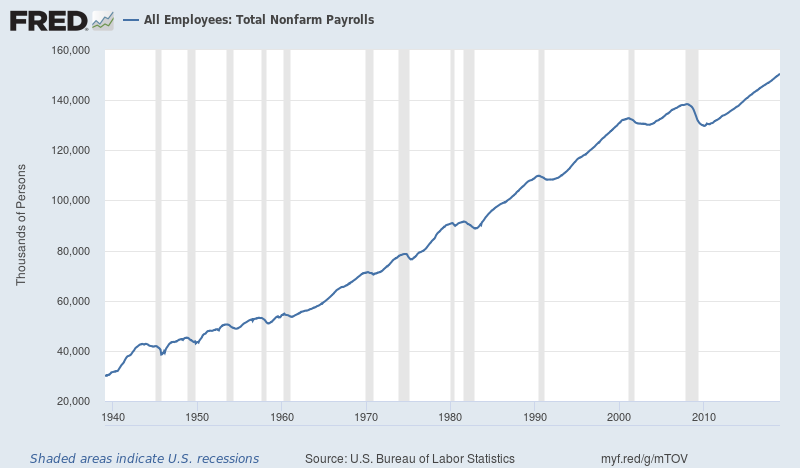
\includegraphics[width=5in]{./resources/nonfarm_level.png}
\end{center}
\end{frame}







\section*{Thanks!}

\end{document}